\documentclass{article}

\title{Advent of Code 2025}
\subtitle{My favorite puzzles from AoC 2025.}
\date{2025-12-27}
\modified{2025-12-27}

\keyword{programming}
\keyword{puzzles}
\keyword{rust}

\begin{document}

\section*

\begin{figure}
  \marginnote{mn-aoc-screen}{A screenshot of the 2025 event page.}
  \includegraphics{/images/46-aoc-2025.webp}
\end{figure}

Advent of Code 2025 lasted only \href{https://adventofcode.com/2025/about#faq_num_days}{12 days}.
I liked the shorter format since keeping up with puzzles for over three weeks in previous years was challenging.

This year I solved the puzzles in \href{https://rust-lang.org/}{Rust}
since I didn't have the capacity to practice a new language.
Rust is a great fit for Advent of Code:
the tooling is mature
and the standard library is rich,
so I didn't need external dependencies\sidenote{sn-z3-dependency}{
  I used \href{https://crates.io/crates/z3}{\code{z3}} to solve part two of \href{#day-10}{day 10},
  which was painful,
  but then I found \href{#tenthmascot-solution}{a way} to solve it without external dependencies.
}.

This article explains solutions to the puzzles I liked the most.

\section{day-03}{Day 3: Lobby}

\href{https://adventofcode.com/2025/day/3}{This puzzle} asks us to find a string subsequence of length $k$ that has the largest numeric value. For example,
if $k = 2$ and the input is \code{818181\b{9}1111\b{2}111}, the output is \code{92}.

In the first part, $k = 2$ and the string length is $n = 100$,
so a brute-force $O(n^2)$ algorithm is fast enough.
The second part increases $k$ to $12$,
so a brute-force algorithm needs to check $\binom{100}{12} = 1,050,421,051,106,700$ \href{https://en.wikipedia.org/wiki/Binomial_coefficient}{combinations}.
Even if it processes a combination in 100 nanoseconds,
it needs over three years to solve one instance.

The shape of this combinatorial explosion is also a clue to the solution.
Binomial coefficients obey a recurrence relation that can be computed using \href{https://en.wikipedia.org/wiki/Dynamic_programming}{dynamic programming}.

\[\binom{n}{k} = \binom{n-1}{k} + \binom{n-1}{k-1}\]

Similarly,
if we define $B$ to be the input string
and $M\left[k, i\right]$ to be the maximum numeric value of length $k$
we can draw from $B\left[0\ldots i\right]$,
we get the following recurrence:

\[M\left[k, i\right] = \operatorname{max}\left\{M\left[k, i-1\right], 10 \times M\left[k-1, i-1\right] + B\left[i-1\right]\right\}\]

Together with boundary conditions $M\left[k, 0\right] = 0$ and $M\left[0, i\right] = 0$, this translates to the following $O(n \times k)$ solution:

\begin{figure}
\begin{code}[rust]
fn max\_numeric\_subsequence(b: &[u8], max\_k: usize) -> u64 {
    let n = b.len();
    let mut m = vec![vec![0; n + 1]; max\_k + 1];
    for k in 1..=max\_k {
        for i in 1..=n {
            m[k][i] = m[k][i-1].max(10 * m[k-1][i-1] + b[i-1] as u64);
        }
    }
    m[k][n]
}
\end{code}
\end{figure}

\section{day-07}{Day 7: Laboratories}

\href{https://adventofcode.com/2025/day/7}{This puzzle} asks us to simulate beam propagation.
The beam starts at the top and splits into two beams each time it reaches a \emph{splitter}.
The first part asks us to count how many splitters the beam reaches;
the second part asks how many paths the beam can take through the maze.

\begin{figure}[center]
\includegraphics{/images/46-day07.gif}
\end{figure}

My programming career started with physics simulations,
which remain close to my heart.
I also like how the second part connects to \href{#day-11}{day 11}.

My solution computes answers to both parts in one grid traversal.
It treats the grid as a \href{https://en.wikipedia.org/wiki/Directed_acyclic_graph}{directed acyclic graph}
in which each space is a parent of the space below it,
and a space above a splitter is a parent of the two spaces on the splitter's sides.
The number of paths to a space is the sum of paths to its parents.

\begin{figure}
\begin{code}
fn count\_splits\_and\_timelines(g: &[Vec<char>]) -> (usize, usize) {
    let n = g.len();
    let m = g[0].len();
    let mut ts = vec![vec![0; m]; n];
    let s = g[0]
        .iter()
        .position(|c| *c == 'S')
        .expect("the first row should have the starting position");
    ts[0][s] = 1;

    let mut splits = 0;
    for i in 1..n {
        for (j, c) in g[i].iter().enumerate() {
            let t = ts[i - 1][j];
            if *c == '^' && t > 0 {
                splits += 1;
                if j > 0 {
                    ts[i][j - 1] += t;
                }
                if j < m - 1 {
                    ts[i][j + 1] += t;
                }
            } else {
                ts[i][j] += t;
            }
        }
    }
    let timelines = ts[n - 1].iter().sum::<usize>();
    (splits, timelines)
}

\end{code}
\end{figure}


\section{day-08}{Day 8: Playground}

\href{https://adventofcode.com/2025/day/8}{This puzzle} gives us a set of \textsc{3d} points
and asks us to repeatedly add an edge between the pair of closest unconnected points.
In the first part,
we must compute the sizes of the three largest
\href{https://en.wikipedia.org/wiki/Component_(graph_theory)}{connected components}
after adding a thousand edges.
In the second part,
we must stop at the first edge that makes the graph fully connected.

I like this puzzle because it's a perfect use case for one of my favorite data structures:
\href{https://en.wikipedia.org/wiki/Disjoint-set_data_structure}{union-find forest}\sidenote{sn-fenwick-tree}{
  My best-loved data structure is \href{https://en.wikipedia.org/wiki/Fenwick_tree}{Fenwick tree}.
}.
This data structure maintains disjoint set partitions and allows merging them efficiently.
In this problem,
the set is the collection of points,
the partitions are connected components,
and merging joins components by adding an edge.

Here is my simple implementation of union-find:

\begin{code}[rust]
struct UnionFind {
    parent: Vec<usize>,
    size: Vec<usize>,
    trees: usize,
}

impl UnionFind {
    fn new(n: usize) -> Self {
        Self {
            parent: (0..n).collect(),
            size: vec![1; n],
            trees: n,
        }
    }

    \emph{/// Returns the root node of node X.}
    \emph{/// Nodes that belong to the same partition share the root.}
    fn find(&self, mut x: usize) -> usize {
        while self.parent[x] != x {
            x = self.parent[x];
        }
        x
    }

    \emph{/// Joins partitions to which nodes X and Y belong.}
    \emph{/// Returns the root of the resulting partition.}
    fn union(&mut self, x: usize, y: usize) -> usize {
        let root\_x = self.find(x);
        let root\_y = self.find(y);
        if root\_x != root\_y {
            let (p, c) = if self.size[root\_x] >= self.size[root\_y] {
                (root\_x, root\_y)
            } else {
                (root\_y, root\_x)
            };
            self.trees -= 1;
            self.parent[c] = p;
            self.size[p] += self.size[c];
            p
        } else {
            root_x
        }
    }

    \emph{/// Returns the size of the partition to which X belongs. }
    fn size(&self, x: usize) -> usize {
        self.size[self.find(x)]
    }

    \emph{/// Returns the partition count.}
    fn tree\_count(&self) -> usize {
        self.trees
    }
}
\end{code}

Both parts require computing all edges between points
and sorting them by distance.

\begin{code}
type Point = (i64, i64, i64);
type Dist = i64;
type Node = usize;

\emph{/// Returns the squared distance between two points.}
fn dist2(a: &Point, b: &Point) -> Dist {
    let dx = a.0 - b.0;
    let dy = a.1 - b.1;
    let dz = a.2 - b.2;
    dx * dx + dy * dy + dz * dz
}

\emph{/// Returns the graph edges sorted by distance.}
fn sorted\_edges(boxes: &[Point]) -> Vec<(Dist, Node, Node)> {
    let n = boxes.len();
    let mut edges = vec![];
    for i in 0..n {
        for j in i + 1..n {
            edges.push((dist2(&boxes[i], &boxes[j]), i, j))
        }
    }
    edges.sort\_by\_key(|e| e.0);
    edges
}
\end{code}

In the first part,
we must compute the sizes of the three largest connected components
after adding \code{top\_k} edges.
We don't have to traverse the graph
because union-find already tracks all the information we need.

\begin{code}
fn part1(boxes: &[Point], top\_k: usize) -> usize {
    let edges = sorted\_edges(boxes);
    let n = boxes.len();
    let mut uf = UnionFind::new(n);

    for (_, i, j) in &edges[0..top\_k] {
        uf.union(*i, *j);
    }

    let mut sizes: Vec<_> = (0..n)
        .filter\_map(|i| (i == uf.find(i)).then\_some(uf.size(i)))
        .collect();
    sizes.sort\_by(|a, b| b.cmp(a));
    
    sizes[0..3].iter().product::<usize>()
}
\end{code}

In the second part,
we must multiply the x-coordinates of the first edge that makes the graph connected.
Union-find makes this trivial.

\begin{code}
fn part2(boxes: &[Point]) -> i64 {
    let mut uf = UnionFind::new(boxes.len());
    let edges = sorted\_edges(boxes);
    for (_, i, j) in &edges {
        uf.union(*i, *j);
        if uf.tree\_count() == 1 {
            return boxes[*i].0 * boxes[*j].0;
        }
    }
    unreachable!()
}
\end{code}

\section{day-09}{Day 9: Movie theater}

In \href{https://adventofcode.com/2025/day/9}{this puzzle},
we work with a \textsc{2d} polygon whose edges are either vertical or horizontal.
In the first part,
we must find the largest rectangle
whose opposite corners coincide with polygon corners.
In the second part,
we must restrict our search to rectangles fully contained within the polygon.

My computational geometry skills are poor,
so I struggled with the second part,
but I also learned much in the process.

I used the same driver function for both parts.
It enumerates all candidate rectangles,
checks that they satisfy a predicate passed as an argument,
and selects the one with the largest area.
For the first part,
the predicate always returns \code{true}.
For the second part,
the predicate checks whether the polygon contains the rectangle.

\begin{code}
type Point = (i64, i64);

fn largest\_rectangle(
    coords: &[Point],
    p: impl Fn(usize, usize, &[Point]) -> bool,
) -> i64 {
    let n = coords.len();
    let mut max\_area = 0;
    for i in 0..n {
        for j in (i + 1)..n {
            if !p(i, j, coords) {
                continue;
            }
            let (x1, y1) = coords[i];
            let (x2, y2) = coords[j];
            let area = ((x2 - x1).abs() + 1) * ((y2 - y1).abs() + 1);
            max\_area = max\_area.max(area);
        }
    }
    max\_area
}
\end{code}

Now the juicy part:
how do we check whether a polygon contains a rectangle?
We must verify two conditions:
\begin{enumerate}
\item The polygon contains all the rectangle's corners.
  Since two corners come from the polygon,
  we only need to check the other two.
\item None of the rectangle's edges cross any polygon edge.
\end{enumerate}

\begin{code}
fn rect\_in\_polygon(a: usize, b: usize, coords: &[Point]) -> bool {
    let (x1, y1) = coords[a];
    let (x2, y2) = coords[b];
    let c = (x1, y2);
    let d = (x2, y1);
    point\_in\_polygon(c, coords)
        && point\_in\_polygon(d, coords)
        && !line\_crosses\_polygon(coords[a], c, coords)
        && !line\_crosses\_polygon(coords[a], d, coords)
        && !line\_crosses\_polygon(coords[b], c, coords)
        && !line\_crosses\_polygon(coords[b], d, coords)
}
\end{code}

To check whether a polygon contains a point,
I used a simplified version of the \href{https://en.wikipedia.org/wiki/Point_in_polygon#Ray_casting_algorithm}{ray casting algorithm}.
It casts a horizontal ray from the point
and counts how many polygon edges the ray crosses.
If this number is odd,
the point lies within the polygon.

\begin{figure}[grayscale-diagram]
\marginnote{mn-ray-intersection}{
   A horizontal ray from point $(x, y)$ intersecting a vertical polygon edge.
}
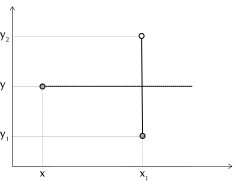
\includegraphics{/images/46-ray-intersection.svg}
\end{figure}

\begin{code}
\emph{/// Checks whether a point lies in a polygon.}
fn point\_in\_polygon(p: Point, vertices: &[Point]) -> bool {
    let mut inside = false;
    let n = vertices.len();
    let (x, y) = p;
    for i in 0..n {
        let (x1, y1) = vertices[i];
        let (_,  y2) = vertices[(i + 1) \% n];
        if (y < y1) != (y < y2) && x1 >= x {
            inside = !inside;
        }
    }
    inside
}
\end{code}

The \code{(y < y1) != (y < y2)} condition is subtle and somewhat cryptic.
It's equivalent to the more verbose \code{y1.min(y2) <= y \&\& y < y1.max(y2)}.
The asymmetric inequality (only one bound is inclusive) ensures
that the edge is vertical (\code{y1 != y2})
and that we don't double-count intersections at polygon corners.

To test whether two lines cross,
we check that the x-coordinate of a vertical line lies between the x-coordinates of a horizontal line, and vice versa.
Note that the lines must \emph{cross}, not just \emph{touch}
(hence the strong inequalities in \code{lines\_cross}).

\begin{figure}[grayscale-diagram]
\marginnote{mn-lines-cross}{
   Horizontal line a-b crossing vertical line c-d.
}
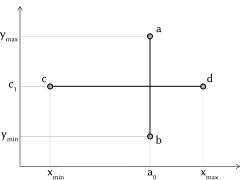
\includegraphics{/images/46-lines-cross.svg}
\end{figure}

\begin{code}
\emph{/// Checks whether line a-b crosses line c-d.}
\emph{/// Both lines must be parallel to one of the axis.}
fn lines\_cross(a: Point, b: Point, c: Point, d: Point) -> bool {
    match (a.0 == b.0, c.0 == d.0) {
        (true, true) => false, \emph{// both vertical}
        (true, false) => {
            \emph{// a-b is vertical, c-d is horizontal}
            assert\_eq!(c.1, d.1);
            let xmin = c.0.min(d.0);
            let xmax = c.0.max(d.0);
            let ymin = a.1.min(b.1);
            let ymax = a.1.max(b.1);
            xmin < a.0 && a.0 < xmax && ymin < c.1 && c.1 < ymax
        }
        (false, true) => lines\_cross(c, d, a, b),
        (false, false) => false, \emph{// both horizontal}
    }
}

\emph{/// Checks whether line a-b crosses any of the polygon edges.}
fn line\_crosses\_polygon(a: Point, b: Point, vertices: &[Point]) -> bool {
    let n = vertices.len();
    for i in 0..n {
        let c = vertices[i];
        let d = vertices[(i + 1) \% n];
        if lines\_cross(a, b, c, d) {
            return true;
        }
    }
    false
}
\end{code}

\section{day-10}{Day 10: Factory}

\href{https://adventofcode.com/2025/day/10}{This puzzle} is the most elaborate of the entire event.
I think of it in terms of vectors.
We start with a set of $n$ $m$-dimensional bit vectors $B = \left\{b_1, \ldots, b_n\right\}$\sidenote{sn-b-buttons}{
  $B$ stands for ``buttons''.
}.

\[b_i = \left(x_1, \ldots, x_m\right), x_j \in \left\{0, 1\right\}\]

The first part of the puzzle gives us a target \emph{binary} vector $t$
and asks us to find integer coefficients $k_i$ such that:

\[k_1 b_1 \oplus \ldots \oplus k_n b_n = t\]

Furthermore, we must minimize the sum $\sum_{1 \leq i \leq n} k_i$.
In other words,
we must find the smallest subset of vectors $b_i$
that yields $t$ when \href{https://en.wikipedia.org/wiki/Exclusive_or}{xored}.

My first instinct was to treat this as a shortest path problem in a state graph.
The vertices correspond to current xor sums,
and edges correspond to vector additions ($\oplus b_i$).
The search starts at the zero vector and must reach $t$.
Since the number of dimensions is small (up to ten),
I represent vectors as 64-bit integers.

\begin{code}
fn lights\_min\_presses(buttons: &[u64], target: u64) -> usize {
    if target == 0 {
        return 0;
    }
    let mut visited: HashSet<u64> = HashSet::new();
    let mut q = VecDeque::new();
    let start = 0;
    visited.insert(start);
    q.push\_back((start, 0));
    while let Some((v, dist)) = q.pop\_front() {
        for b in buttons {
            let s = v ^ *b;
            if visited.contains(&s) {
                continue;
            }
            if s == target {
                return dist + 1;
            }
            visited.insert(s);
            q.push\_back((s, dist + 1));
        }
    }
    panic!("Target state is unreachable: {buttons:?} {target}");
}
\end{code}

The second part has the same structure,
but uses normal addition instead of xor,
and the target vector can contain arbitrary non-negative integers.
The objective remains minimizing the sum of coefficients $k_i$.

\[k_1 b_1 + \ldots + k_n b_n = t\]

I tried adapting the graph-search solution
and explored dynamic programming techniques,
but nothing worked.
The values in the target vector were too large (over 50 on average in my input) for my programs to finish in reasonable time.

Like \href{https://www.reddit.com/r/adventofcode/comments/1pivlyh/2025_day_10_every_time_a_problem_looks_remotely/}{many solvers},
I resorted to the \textsc{smt} solver \href{https://github.com/Z3Prover/z3}{z3}.
Rust has \href{https://crates.io/crates/z3}{nice bindings},
and my code worked on the first try.

\begin{code}
fn joltage\_min\_presses\_z3
    ndims: usize,
    buttons: &[u64],
    target: &[u16],
) -> usize {
    use z3::{ast::Int, Optimize, SatResult};
    let opt = Optimize::new();

    \emph{// Define the k\_i variables.}
    let mut vars = vec![];
    for i in 0..buttons.len() {
        let k\_i = Int::fresh\_const(format!("k\_{}", i).as\_str());
        opt.assert(&k\_i.ge(0));
        vars.push(k\_i);
    }

    \emph{// Define a constraint for every dimension.}
    for d in 0..ndims {
        let mut vals = vec![];
        for (i, b) in buttons.iter().enumerate() {
            if *b & (1 << d) > 0 {
                vals.push(vars[i].clone());
            }
        }
        opt.assert(&Int::add(&vals).eq(target[d]));
    }

    \emph{// Minimize the sum of k\_i.}
    opt.minimize(&Int::add(&vars));

    let mut result = 0;
    match opt.check(&[]) {
        SatResult::Sat => {
            let model = opt.get\_model().unwrap();
            for v in vars.iter() {
                let val = model
                    .get\_const\_interp(v)
                    .unwrap()
                    .as\_i64()
                    .unwrap();
                result += val as usize;
            }
        }
        \_ => {
            panic!("No solution found.");
        }
    }
    result
}
\end{code}

\subsection{tenthmascot-solution}{Divide and conquer}

The z3 solution feels unsatisfactory:
I didn't become any wiser\sidenote{sn-z3-is-awesome}{
  Except for learning that z3 is awesome, of course.
}, and my compile times exploded.
Luckily, Reddit user \href{https://www.reddit.com/user/tenthmascot/}{u/tenthmascot}
\href{https://www.reddit.com/r/adventofcode/comments/1pk87hl/2025_day_10_part_2_bifurcate_your_way_to_victory/}{posted an ingenious solution}
that was fast and didn't require any dependencies.

The solution relies on this observation:
if all $k_i$ are even ($k_i = 2 k_i^\prime$),
then each component in the target vector must also be even.
We can halve both the coefficients and the target
to get a smaller instance of the same problem,
reducing the search space.

\[ \left(2 k_1^\prime \times b_1 + \ldots + 2 k_n^\prime b_n = 2 t^\prime \right) \Rightarrow \left( k_1^\prime b_1 + \ldots + k_n^\prime b_n = t^\prime \right)\]

We can't be sure all $k_i$ are even,
but we can make them even by subtracting at most one.
Which $k_i$ should we decrement?
We don't know, so we try all $2^n$ combinations and pick the best result!

Unfortunately, testing all combinations every time is still too slow.
Naive approaches must evaluate around $50^n$ combinations
(where $50$ is a typical value from the target vector).
Our ``clever'' way probes\ldots  $(2^n)^{\log_2 50} = 50^n$ combinations.

Luckily, we can do better:
restrict the search to combinations matching the target's parity.
If an equation holds under normal arithmetic,
it must also hold modulo two.

\[ \left( k_1 b_1 + \ldots + k_n b_n = t \right) \Rightarrow  \left( \left(k_1 \oplus 2\right) b_1 \oplus \ldots \oplus \left(k_n \oplus 2\right) b_n = t \oplus 2 \right)\]


For example, if the target vector is $\left(32, 93, 66, 72, 61\right)$,
its parity vector is $\left(0, 1, 0, 0, 1\right)$,
and we need to consider only those combinations of $b_i$
that yield the same parity when xored.
Now we deal with boolean variables just like we did in the first part,
but this time we must look at all solutions,
not only the optimal one.

If combinations of input vectors $b_i$ cover the parity space uniformly,
we only evaluate about $\frac{2^n}{2^m} = 2^{n-m}$ candidates at each step.
All instances in my input exhibit near-perfect distribution\sidenote{sn-distribution}{
  I wrote a program that generates random vectors and prints their parity group size distributions.
  Uniform coverage seems to be the norm.
}.
To exploit this reduction,
precompute parity groups and consult them at every recursion level.

Here is my implementation of \code{u/tenthmascot}'s idea:

\begin{code}

type ParityGroups = HashMap<u64, Vec<u64>>;

fn parity\_groups(ndims: usize, buttons: &[u64]) -> ParityGroups {
    let n = buttons.len();
    assert!(n <= 64);
    let mut groups = ParityGroups::new();
    \emph{// Use a 64-bit integer to represent subsets.}
    for mask in 0..(1 << ndims) {
        let mut parity\_bits = 0;
        for i in 0..n {
            if mask & (1 << i) == 0 {
                continue;
            }
            for d in 0..ndims {
                if buttons[i] & (1 << d) > 0 {
                    parity\_bits ^= 1 << d;
                }
            }
        }
        groups.entry(parity\_bits).or\_default().push(mask);
    }
    groups
}

fn joltage\_min\_presses
    groups: &ParityGroups,
    buttons: &[u64],
    target: &[u16],
) -> Option<usize> {
    if target.iter().sum::<u16>() == 0 {
        return Some(0);
    }

    \emph{// Compute parity vector of the target.}
    let mut parity = 0u64;
    for (d, t\_d) in target.iter().enumerate() {
        if t\_d & 1 > 0 {
            parity |= 1u64 << d;
        }
    }

    let mut best: Option<usize> = None;

    \emph{// Loop over subsets that give the desired parity.}
    'outer: for subset in groups.get(&parity)? {
        \emph{// Compute the arguments for a smaller problem.}
        let mut new\_target = target.to\_vec();
        let mut presses = 0;
        for i in 0..buttons.len() {
            if subset & (1 << i) == 0 {
                continue;
            }
            presses += 1;
            for d in 0..target.len() {
                if buttons[i] & (1 << d) > 0 {
                    if new\_target[d] == 0 {
                        continue 'outer;
                    }
                    new\_target[d] -= 1;
                }
            }
        }
        for v in new\_target.iter\_mut() {
            assert_eq!(*v \% 2, 0);
            *v /= 2;
        }

        \emph{// Solve the smaller problem recursively.}
        if let Some(x) = joltage\_min\_presses(groups, buttons, &new\_target) {
            let total = presses + 2 * x;
            best = Some(best.map\_or(total, |v| v.min(total)));
        }
    }
    best
}
\end{code}

Parity groups also yield a simple algorithm for part one:
pick the smallest subset in the target's parity group.

\begin{code}
fn lights\_min\_presses\_parity(groups: &ParityGroups, target: u64) -> usize {
    groups
        .get(&target)
        .expect("no solution found")
        .iter()
        .map(|mask| mask.count\_ones() as usize)
        .min()
        .unwrap()
}
\end{code}

\section{day-11}{Day 11: Reactor}

\href{https://adventofcode.com/2025/day/11}{This puzzle} asks us to count paths between two vertices in a \href{https://en.wikipedia.org/wiki/Directed_acyclic_graph}{directed acyclic graph}.
That's the same problem as \href{#day-07}{day seven} part two,
but this time the graph is general, not grid-embedded.
On day seven, the grid structure provided a natural topological order.
Here, we must compute it ourselves.

\begin{code}
type Graph = Vec<Vec<usize>>;
  
\emph{/// Returns the vertices of a graph in a topological order.}
fn toposort(g: &Graph, start: usize) -> Vec<usize> {
    fn go(
        g: &Graph,
        v: usize,
        visited: &mut Vec<bool>,
        out: &mut Vec<usize>,
    ) {
        if visited[v] {
            return;
        }
        visited[v] = true;
        for w in &g[v] {
            go(g, *w, visited, out);
        }
        out.push(v);
    }

    let mut out = vec![];
    let mut visited = vec![false; g.len()];
    go(g, start, &mut visited, &mut out);
    out.reverse();
    out
}

\emph{/// Computes the number of paths between two vertices.}
fn count\_paths(g: &Graph, start: usize, end: usize) -> usize {
    let mut d = vec![0; g.len()];
    d[start] = 1;
    for p in toposort(g, start) {
        for c in &g[p] {
            d[*c] += d[p];
        }
    }
    d[end]
}
\end{code}

In the second part,
we must count paths from \code{svr} to \code{out}
that pass through both \code{fft} and \code{dac} (in any order).
The straightforward solution multiplies path counts for segments
\code{svr -> fft -> dac -> out} and \code{svr -> dac -> fft -> out}.

\begin{code}
let fft\_dac =
    count\_paths(&g, svr, fft) *
    count\_paths(&g, fft, dac) *
    count\_paths(&g, dac, out);
let dac\_fft =
    count\_paths(&g, svr, dac) *
    count\_paths(&g, dac, fft) *
    count\_paths(&g, fft, out);
println!("{}", fft\_dac + dac\_fft);
\end{code}

Of course, only one of \code{count\_paths(\&g, dac, fft)} and \code{count\_paths(\&g, fft, dac)}
can be non-zero.

\section{day-12}{Day 12: Christmas tree farm}

\href{https://adventofcode.com/2025/day/12}{This puzzle} asks
whether a rectangle of given dimensions can fit a set of irregular tiles.
The problem seemed overwhelmingly complex and the input sizes were large,
so I suspected a trick.
After all, the final day is often cheesy.

One smoke test for whether a rectangle can fit a set of tiles
is checking whether its area is large enough.
If the rectangle's area is 360 units
and the tiles occupy 365 units,
the instance is clearly unsolvable.

I printed area ratios for all instances in my input.
They fell into two groups:
ratios <80\% and ratios >100\%.
I assumed that if a rectangle \emph{could} fit the tiles,
it did.
Luckily, this guess was correct.

My solution boils down to the following humble heuristic:

\begin{code}
let tiles\_per\_shape: Vec<usize> =
    shapes.iter().map(|g| grid\_count(g, &'#')).collect();

let mut total = 0usize;
for instance in instances {
    let tile\_count = tiles\_per\_shape
        .iter()
        .zip(instance.shape\_counts.iter())
        .map(|(x, y)| x * y)
        .sum::<usize>();

    if tile\_count <= instance.w * instance.h {
        total += 1;
    }
}
println!("{total}");
  
\end{code}

\end{document}



